\documentclass[tikz,border=0mm]{standalone}
\usepackage{tikz}
\usetikzlibrary{positioning}
\tikzset{
    mynodee/.style={minimum height=0mm, minimum width=0mm, inner sep=0mm
  },
  mynode/.style={
    draw, circle, minimum height=1.7mm, minimum  width=1.7mm,line width=0.5mm
  },
  rect/.style={
    draw, rectangle, rounded corners, minimum height=7mm, minimum  width=30mm,line
    width=0.5mm, dotted
  }
}

\begin{document}

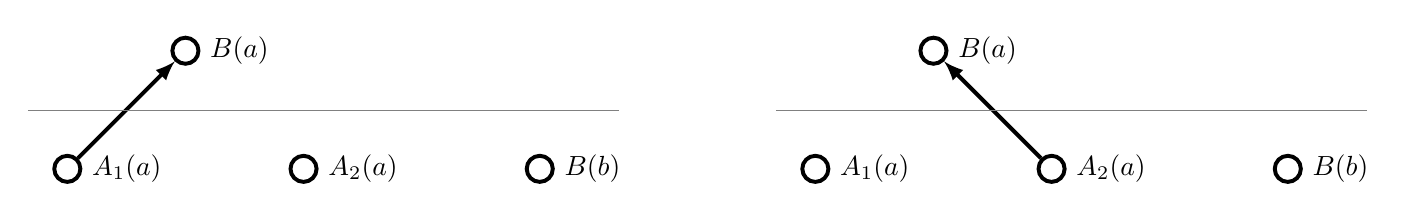
\begin{tikzpicture}
  \begin{scope}
   \node[mynode, label=right:$A_1(a)$] (a1a) at (0, 0) {};
   \node[mynode, label=right:$A_2(a)$] (a2a) at (3, 0) {};
   \node[mynode, label=right:$B(b)$] (bb) at (6, 0) {};
   \node[mynode, label=right:$B(a)$] (ba) at (1.5, 1.5) {};

   \draw[-latex,line width=0.5mm] (a1a) -- (ba);
   \draw[very thin,gray] (-.5, .75) -- (7, .75);
 \end{scope}
  \begin{scope}[xshift=9.5cm]
   \node[mynode, label=right:$A_1(a)$] (a1a) at (0, 0) {};
   \node[mynode, label=right:$A_2(a)$] (a2a) at (3, 0) {};
   \node[mynode, label=right:$B(b)$] (bb) at (6, 0) {};
   \node[mynode, label=right:$B(a)$] (ba) at (1.5, 1.5) {};

   \draw[-latex,line width=0.5mm] (a2a) -- (ba);
   \draw[very thin,gray] (-.5, .75) -- (7, .75);
 \end{scope}
\end{tikzpicture}

\end{document}

%%% Local Variables:
%%% mode: latex
%%% TeX-master: "fig-matgraph"
%%% End:


